\documentclass[12pt,letterpaper]{article}
\usepackage[left=2.5cm,right=2.5cm,top=3cm,bottom=2cm]{geometry}
\usepackage[utf8]{inputenc}
\usepackage[spanish, es-tabla]{babel}
\usepackage[version=3]{mhchem}
\usepackage[journal=jacs]{chemstyle}
\usepackage{amsmath}
\usepackage{amsfonts}
\usepackage{amssymb}
\usepackage{makeidx}
\usepackage{xcolor}
\usepackage[stable]{footmisc}
\usepackage[section]{placeins}
\usepackage{listings}
\usepackage{graphicx} 
%Paquetes necesarios para tablas
\usepackage{longtable}
\usepackage{array}
\usepackage{xtab}
\usepackage{multirow}
\usepackage{colortab}
%Paquete para el manejo de las unidades
\usepackage{siunitx}
\sisetup{mode=text, output-decimal-marker = {,}, per-mode = symbol, qualifier-mode = phrase, qualifier-phrase = { de }, list-units = brackets, range-units = brackets, range-phrase = --}
\DeclareSIUnit[number-unit-product = \;] \atmosphere{atm}
\DeclareSIUnit[number-unit-product = \;] \pound{lb}
\DeclareSIUnit[number-unit-product = \;] \inch{"}
\DeclareSIUnit[number-unit-product = \;] \foot{ft}
\DeclareSIUnit[number-unit-product = \;] \yard{yd}
\DeclareSIUnit[number-unit-product = \;] \mile{mi}
\DeclareSIUnit[number-unit-product = \;] \pint{pt}
\DeclareSIUnit[number-unit-product = \;] \quart{qt}
\DeclareSIUnit[number-unit-product = \;] \flounce{fl-oz}
\DeclareSIUnit[number-unit-product = \;] \ounce{oz}
\DeclareSIUnit[number-unit-product = \;] \degreeFahrenheit{\SIUnitSymbolDegree F}
\DeclareSIUnit[number-unit-product = \;] \degreeRankine{\SIUnitSymbolDegree R}
\DeclareSIUnit[number-unit-product = \;] \usgallon{galón}
\DeclareSIUnit[number-unit-product = \;] \uma{uma}
\DeclareSIUnit[number-unit-product = \;] \ppm{ppm}
\DeclareSIUnit[number-unit-product = \;] \eqg{eq-g}
\DeclareSIUnit[number-unit-product = \;] \normal{\eqg\per\liter\of{solución}}
\DeclareSIUnit[number-unit-product = \;] \molal{\mole\per\kilo\gram\of{solvente}}
\usepackage{cancel}
%Paquetes necesarios para imágenes, pies de página, etc.
\usepackage{graphicx}
\usepackage{lmodern}
\usepackage{fancyhdr}
%Instrucción para evitar la indentación
%\setlength\parindent{0pt}
%Paquete para incluir la bibliografía
\usepackage[backend=biber]{biblatex}
\bibliography{ref.bib}

%Formato del título de las secciones

\usepackage{titlesec}
\usepackage{enumitem}
\titleformat*{\section}{\bfseries\large}
\titleformat*{\subsection}{\bfseries\normalsize}

%Creación del ambiente anexos
\usepackage{float}
\floatstyle{plaintop}
\newfloat{anexo}{thp}{anx}
\floatname{anexo}{Anexo}
\restylefloat{anexo}
\restylefloat{figure}

%Modificación del formato de los captions
\usepackage[margin=10pt,labelfont=bf]{caption}

%Paquete para incluir comentarios
\usepackage{todonotes}

%Paquete para incluir hipervínculos
\usepackage[colorlinks=true, 
            linkcolor = blue,
            urlcolor  = blue,
            citecolor = black,
            anchorcolor = blue]{hyperref}

%%%%%%%%%%%%%%%%%%%%%%
%Inicio del documento%
%%%%%%%%%%%%%%%%%%%%%%

\begin{document}
\renewcommand{\labelitemi}{$\checkmark$}

\renewcommand{\CancelColor}{\color{red}}

\newcolumntype{L}[1]{>{\raggedright\let\newline\\\arraybackslash}m{#1}}

\newcolumntype{C}[1]{>{\centering\let\newline\\\arraybackslash}m{#1}}

\newcolumntype{R}[1]{>{\raggedleft\let\newline\\\arraybackslash}m{#1}}

\renewcommand{\thesection}{\Roman{section}}

\begin{center}
	\textbf{\LARGE{Análisis sobre distintas bases de datos}}\\
	\vspace{7mm}
		\textbf{\large{Ivan Arat Duran Ramírez}}\\
		\textbf{\normalsize{NUA: 391411}}\\
	\vspace{4mm}
	\textbf{\large{Herramientas Informáticas y Gestión de la Información}}\\
	\today
\end{center}

\vspace{7mm}

\section*{\centering Resumen}

Se realizó una predicción sobre la lista nominal de México en febrero de 2021 mediante la generación de una regresión lineal con los datos de las listas previas, desde septiembre de 2019 hasta diciembre de 2020. Se obtuvo que el total de casillas a instalar será de 6071.\\

Por otro lado, se realizó el análisis de una base de datos distinta. En este caso, un estudio de la mortalidad en la población leonesa. Con los datos de la lista de defunciones en México de los años 2014 a 2018 se intentó predecir el número de muertes a causa de infartos al miocardio y diabetes en 2019, obteniendo 939 y 212 contra los 5686 y 249 decesos registrados, respectivamente.

\section*{Introducción}
Lo mencionamos en el título del reporte, pero ¿qué es una base de datos? Entendamos por base de datos al conjunto de información almacenada, perteneciente a un mismo contexto para ser analizada posteriormente. Usualmente las bases de datos son arreglos matriciales, de forma que la información se consulta tomando filas y columnas. En nuestro caso, haremos uso de Python para interpretar toda la información que las bases de datos tienen.\\

\section{Sobre el análisis de la lista nominal}
Para la base de datos "\textit{Estadística de Padrón Electoral y Lista Nominal de Electores}", propuesta por la profesora y obtenida del sitio oficial del Instituto Nacional Electoral (INE)\cite{INE}, se llevaron a cabo las siguientes tareas:

\begin{enumerate}
    \item Filtrar la información de los archivos de modo que sólo tengamos la que corresponde al Estado de Guanajuato. 
    \item Aplicar un nuevo filtro para obtener la información de la lista nominal correspondiente a los municipios y sus respectivas secciones. 
    \item Repetir este proceso para los 16 archivos con los que contamos, correspondientes a los meses desde septiembre de 2019 hasta diciembre de 2020. 
    \item Con la lista nominal recopilada de los 16 archivos, hacer una regresión lineal y predecir la lista nominal a febrero de 2021
    \item Calcular el número de casillas a instalar tanto en los municipios como en las secciones siendo que a cada 750 actas le corresponde 1 casilla. 
\end{enumerate}

Repasaremos el código hecho sección a sección. Se hizo uso de los ciclos for para poder realizar las tareas 1, 2, 4 y 5 de manera casi simultánea, por lo que explicaré de manera general qué fue lo que se hizo. Y antes que todo, estas fueron las bibliotecas empleadas a lo largo del proyecto:
\scriptsize{\begin{lstlisting}[language=Python]
    import pandas as pd 
    import matplotlib.pyplot as plt 
    import numpy as np
    import glob
    from sklearn.linear_model import LinearRegression
    import math as mt
\end{lstlisting}}
\normalsize{Puesto que los archivos del año 2019 tienen una estructura diferente a la de los archivos del año 2020 decidí hacer el análisis en años separados y luego unir los resultados. Primero, cargaremos los archivos en un arreglo con la librería glob:}
\scriptsize{\begin{lstlisting}[language=Python]
    files2019=glob.glob("D:/ProgramasJupyter/HIGI/PrediccionINE/Archivos2019/*.txt")
    files2020=glob.glob("D:/ProgramasJupyter/HIGI/PrediccionINE/Archivos2020/*.txt")
\end{lstlisting}}
\normalsize{Cabe mencionar que, al ser pocos archivos los que se iban a estudiar, decidí renombrarlos manualmente para ubicarlos en orden cronológico dentro de mi directorio. Dicho esto, se escribieron las siguientes líneas:} 
\scriptsize{\begin{lstlisting}[language=Python]
    l_mpo_gral_19=[]
    l_sec_gral_19=[]
    for i in range(0, len(files2019)):
        data_19 = pd.read_csv(files2019[i], usecols=[0,1,2,3,9])
        data_ent_19=data_19[data_19['ENTIDAD']==11]
        mpos_19=np.unique(data_ent_19['MUNICIPIO'])
        secs_19=np.unique(data_ent_19['SECCION'])
        l_mpo_19=[]
        l_sec_19=[]
        for mpo_19 in mpos_19[1:]:
            l_mpo_19.append(data_ent_19[data_ent_19['MUNICIPIO']==mpo_19]['LISTA'].sum())
        l_mpo_gral_19.append(l_mpo_19)
        for sec_19 in secs_19[1:]:
            l_sec_19.append(data_ent_19[data_ent_19['SECCION']==sec_19]['LISTA'].sum())
        
        temp=np.zeros(3161)
        temp[:len(l_sec_19)]=l_sec_19
        l_sec_gral_19.append(temp)
        
    l_mpo_gral_array_19=np.asarray(l_mpo_gral_19)
    
    l_sec_gral_array_19=np.asarray(l_sec_gral_19)
\end{lstlisting}}
\normalsize{Respecto a la variable temp que se muestra en la sección previa. Al avanzar en el proyecto tuve con problemas relacionados a la función np.concatenate puesto que las secciones no tienen el mismo tamaño en todos los años, a diferencia de los municipios. Para poder concatenar los arreglos en una misma matriz era necesario tener arreglos de la misma dimensión así que para resolver el problema decidí revisar los tamaños de las secciones mes con mes y me di cuenta que el mayor era de 3161. Asumí que los meses con menos secciones tendrían todas las secciones previas a 3161, es decir, que eran continuas pero cortadas hasta antes de ese número, por tanto, un arreglo con 3161 ceros sería suficiente para después sustituirlos con los valores reales de la lista en cada sección ya que, al final, sobre estos datos haremos sumas por lo que el cero es un elemento completamente neutro.}\\

\normalsize{Como nota para evitar repetitividad, aquellas variables que tengan un \textit{mpo} o \textit{sec} de por medio corresponden a los datos de los municipios y las secciones, respectivamente. De esta forma, cargamos los archivos en la variable data\_19 y posteriormente filtramos sólo aquellos datos posteriores a la columna $"ENTIDAD"$ con valor 11. Una vez que los tenemos filtrados, las siguientes líneas sirven para indexar en un arreglo los valores de la lista nominal correspondientes a cada municipio y cada sección. Por útlimo, al ser datos extraídos con pandas creí necesario poder analizarlos con NumPy y por tanto, usé la función np.asarray para poder tener arreglos en lugar de listas. El tratamiento para el año 2020 es totalmente análogo a este pero sustituyendo los 19 por 20 y en lugar de la columna "LISTA" (9) se tiene la columna "LISTA\_NAL" (13).\\

Una vez que se llenaron los arreglos con la información necesaria los uní en uno sólo, que sería el arreglo que contendría toda la lista de los municipios y secciones de los 16 archivos, obteniendo una matriz de 16$\times$46 y 16$\times$3161, respectivamente:} 
\scriptsize{\begin{lstlisting}[language=Python]
    mun_total=np.concatenate((l_mpo_gral_array_19,l_mpo_gral_array_20))
    sec_total=np.concatenate((l_sec_gral_array_19,l_sec_gral_array_20))
\end{lstlisting}}
\normalsize{En este punto hemos casi acabado pues, recapitulando, ya hemos filtrado la información de la lista de los municipios y las secciones a lo largo de los 16 meses, por lo que sólo queda realizar una regresión lineal para hacer nuestra predicción. Mostraré las líneas que calculan la regresión lineal para los 46 municipios pero las líneas que lo hacen para las secciones son completamente análogas.}
\scriptsize{\begin{lstlisting}[language=Python]
    x=np.linspace(1,16,16).reshape(-1,1)
    linR=LinearRegression()
    mm=[]
    bm=[]
    predm=[]
    for i in range(46):
        linR.fit(x,mun_total[:,i])
        mm.append(int(linR.coef_[0]))
        bm.append(int(linR.intercept_))
        predm.append(int(linR.predict(np.array(18.0).reshape(1,-1))))
    
    pm=[]
    for i in range(len(predm)):
        am=mt.ceil(predm[i]/750)
        pm.append(am)
        
    pmm=np.asarray(pm)
\end{lstlisting}}
\normalsize{Estas líneas previas no son más que lo que se debe de realizar para poder utilizar LinearRegression de SciKit Learn. Los arreglos que nos interesan son pmm (la predicción de la lista nominal para los municipios) y smm (la predicción de la lista nominal para las secciones). De nuevo se usó np.asarray para poder utilizar la función .sum() y conocer la suma total de la lista prevista para el 2021.\\

Como nota general, puesto que los meses corren en orden cronológico, podemos entender la lista nominal como una función del tiempo donde al primer mes (septiembre de 2019) se le asignó el número 1, a octubre de 2019 el 2 y así sucesivamente hasta diciembre de 2020 con el 16, por lo que para conocer la predicción en febrero de 2021 sería necesario evaluar esta función del tiempo en $t=18$, como se muestra en el script anterior. Además, nótese que el arreglo preds fue dividido en 750, esto porque cada 750 actas le corresponde una casilla. La función mt.ceil() nos ayuda a redondear cualquier decimal al número entero próximo, esto para garantizar que incluso con una cantidad menor a 750 actas pongamos al menos una casilla.}

\small{\subsection*{Resultados y discusiones}}
\normalsize{De acuerdo con las consideraciones que utilizamos para calcular la lista nominal a febrero de 2021 obtuvimos que serían necesarias 6071 casillas. La siguiente tabla muestra las casillas necesarias para cada municipio:}
% Table generated by Excel2LaTeX from sheet 'resultados_INE_mpo'
\begin{table}[H]
  \centering
  \caption{Predicción de las casillas a instalar por municipio}
    \begin{tabular}{rrrr}
    \multicolumn{1}{l}{Estado} & \multicolumn{1}{l}{Predicción} & \multicolumn{1}{l}{Estado} & \multicolumn{1}{l}{Predicción} \\
    1     & 92    & 24    & 15 \\
    2     & 129   & 25    & 77 \\
    3     & 178   & 26    & 63 \\
    4     & 68    & 27    & 291 \\
    5     & 94    & 28    & 113 \\
    6     & 6     & 29    & 39 \\
    7     & 518   & 30    & 113 \\
    8     & 44    & 31    & 128 \\
    9     & 83    & 32    & 83 \\
    10    & 13    & 33    & 124 \\
    11    & 102   & 34    & 6 \\
    12    & 32    & 35    & 84 \\
    13    & 26    & 36    & 9 \\
    14    & 156   & 37    & 188 \\
    15    & 192   & 38    & 14 \\
    16    & 23    & 39    & 42 \\
    17    & 581   & 40    & 19 \\
    18    & 40    & 41    & 68 \\
    19    & 56    & 42    & 157 \\
    20    & 1565  & 43    & 21 \\
    21    & 60    & 44    & 65 \\
    22    & 25    & 45    & 12 \\
    23    & 171   & 46    & 86 \\
    \end{tabular}%
  \label{tab:addlabel}%
\end{table}%
Nótese que si se quiere saber cuántas actas se tendrán por municipio en febrero de 2021, basta con multiplicar cada entrada de la tabla por 750. \\

Podemos confiar en estos resultados si nos basamos en el siguiente gráfico, donde, si bien los datos no se distinguen unos de otros, apreciamos que todas las líneas (las cuales representan la evolución de la lista nominal de los municipios en el tiempo), son rectas, por lo tanto, podemos arriesgarnos a tomar en cuenta una regresión lineal:
\begin{figure}[H]
    \centering
    \includegraphics{RegresiónLinealMpo.png}
    \caption{Evolución temporal de la lista nominal municipio por municipio}
    \label{fig:my_label}
\end{figure}
El gráfico no tiene otro propósito más que el de ser ilustrativo porque, como es evidente, no arroja nada de información cuantitativa sobre nuestro problema.\\

Por otro lado, si hacemos una regresión lineal para cada una de las secciones obtendremos que serían necesarias 7614 casillas. ¿Es este resultado confiable? Como discutimos en la entrega pasada, no. Los datos por sección son mucho más suceptibles a cambios que los datos por municipios, por lo que lo ideal habría sido aplicar la regresión lineal de cada municipio a cada una de las secciones. Sin embargo, no logré implementar un algoritmo que capturara las secciones correspondientes a cada municipio por lo que hacer esto me fue imposible.\\

Con el fin de enseñar la suceptibilidad de las secciones, el siguiente gráfico muestra el comportamiento de las secciones mes con mes.
\begin{figure}[H]
    \centering
    \includegraphics{RegresiónLinealSec.png}
    \caption{Modelado del comportamiento de las secciones mes con mes}
    \label{fig:my_label}
\end{figure}
Como podemos ver, intentar adaptar gran parte de estas gráficas a un modelo lineal no está en lo absoluto justificado, por lo tanto, como resultado final nos quedaremos con que debemos instalar alrededor de 6071 casillas en todo el Estado. \\

\section{Sobre el análisis de las defunciones en México}
Para el caso donde analizamos la base de nuestra elección, hice uso de las actas de defunción registradas en los años 2014 a 2019 en México del sitio oficial del Gobierno de México, específicamente de la sección de datos abiertos \cite{Defunciones}. Me propuse resolver lo siguiente:  
\begin{enumerate}
    \item Filtrar la información de los archivos de modo que sólo tengamos la que corresponde a León. 
    \item Aplicar un nuevo filtro para obtener la información de las causas de muerte registradas en ese año.  
    \item Repetir este proceso para los años 2014 a 2018.
    \item Con los datos de las defunciones registras, predecir el número de decesos que se registraron en 2019 por 3 causas de muerte distintas. 
\end{enumerate}

Las bilbiotecas empleadas en para analizar esta base de datos es la misma que la que se usó para el INE. Los archivos fueron nombrados igualmente en orden alfabético para poder analizarlos cronológicamente 
\scriptsize{\begin{lstlisting}[language=Python]
    mun_t = []
    causa_t = []
    mes_t=[]
    for i in range(0,len(files)):
        data = pd.read_csv(files[i], usecols=[0,1,10,18])
        estado = data[data['ent_regis']==11]
        mpo = estado[estado['mun_regis']==20]
        causa = list(mpo['causa_def'])
        causa_t.append(causa)
\end{lstlisting}}
\normalsize{En esta sección de código lo que se hizo fue filtrar de todos los archivos las columnas que contenían la información de las causas de muerte en León. Es imporante recalcar que aquí no usamos la función unique porque a cada deceso registrado se le otorga una nueva fila en la base de datos, por lo que nos interesa que se repitan las causas para poder contabilizar todas las defunciones.}\\

Esta sección es muy sencilla, de manera análoga a lo que hicimos en el INE, transformamos nuestras listas en arrays. Además, puesto que cada entrada corresponde a una defunción, basta con conocer la longitud del arreglo para saber cuántas defunciones se registraron año con año dada una causa de muerte:
\scriptsize{\begin{lstlisting}[language=Python]
    causa_a = np.asarray(causa_t, dtype=object )
    total_leon = []
    for i in range(0,5):
        total_leon.append(len(causa_t[i]))
        
    totals=np.asarray(total_leon)
    print(totals.sum())
\end{lstlisting}}
\normalsize{Después, decidí qué causas de muerte quería estudiar. La primera, era la causa más común en todo México, la cual obtuve de una búsqueda en Google y resultó ser un infarto al miocardio, la segunda fue una causa de muerte al azar de entre las que se registraron y obtuve el Síndrome de Dressler y por último obtuve la moda del arreglo que contenía las causas de muerte, la cual es la causa de muerte más común entre los leoneses y obtuve que fue la diabetes.}\\

Para saber cuántas personas murieron por cada una de esas causas utilicé un contador, de esta forma podía saber cuántas veces se repetían las muertes por determinada causa. Cabe aclarar que las causas de muerte vienen especificadas en un catálogo con un código alfanumérico, en el caso del infarto al miocardio es el código I219, para el síndrome de Dressler, I241 y para la diabetes el E119.
\scriptsize{\begin{lstlisting}[language=Python]
    imoda=[]
    for i in range(5):
        imoda.append(causa_t[i].count('I219'))
    print(imoda)
    
    dmoda=[]
    for i in range(5):
        dmoda.append(causa_t[i].count('I241'))
    print(dmoda)
    
    mmoda=[]
    for i in range(5):
        mmoda.append(causa_t[i].count('E119'))
\end{lstlisting}}
\normalsize{Nótese que los arreglos obtenidos previamente guardan el número de decesos asociados a una causa de muerte, por tanto, ya tenemos los datos suficientes para general una regresión lineal.}
\scriptsize{\begin{lstlisting}[language=Python]
    xi = np.linspace(1,5,5).reshape(-1,1)
    lri = LinearRegression()
    lri.fit(xi,imoda)
    mi = lri.coef_[0]
    bi = lri.intercept_
    xi_p = list(lri.predict(np.array(6).reshape(1,-1)))
\end{lstlisting}}
\normalsize{Este script se modificó para cada una de las causas de muerte, pero todas conservan el mismo algoritmo.}\\

Por último, para investigar más sobre la base, decidí tratar de predecir el número de muertes registradas en 2019, por lo que cargué la información nuevamente pero ahora sin ningún filtro de búsqueda y conté las entradas de las causas de muertes totales. Con esto tenía los datos suficientes para hacer mi regresión lineal: 
\scriptsize{\begin{lstlisting}[language=Python]
    muerte = []
    for i in range(0,5):
        dataa = pd.read_csv(files[i], usecols=[0,1,10,18])
        muerte.append(len(dataa['causa_def']))
        
    x = np.linspace(1,5,5).reshape(-1,1)    
    lrm = LinearRegression()
    lrm.fit(x,muerte)
    p = lrm.predict(np.array(6.0).reshape(1,-1))
\end{lstlisting}}
\normalsize{
\subsection*{\small{Resultados y Discusiones}}
Como parte del proyecto se nos fue solicitado la elaboración de una presentación que contuviera los resultados de nuestra investigación. A medida que esta fue elaborarada, me percaté que había mucha información que podía obtener dentro de esta base de datos. A continuación voy a describir toda la información que uno puede inferir:} 

\begin{itemize}
    \item \textbf{Las muertes totales en México: }
\end{itemize}
Obtuve que en los años 2014 a 2018 fallecieron 633641, 655688, 685766, 703047 personas, respectivamente. Con estos datos al aplicar una regresión lineal se obtuvo que en 2019 fallecerían 747741 personas, cuando el dato reportado por el INEGI fue de 747784. En el siguiente gráfico podemos ver cómo el comportamiento es muy similar a una recta: 
\begin{figure}[H]
    \centering
    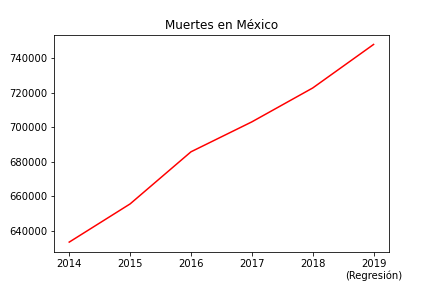
\includegraphics[scale=0.8]{ModeloMuertes.png}
    \caption{Modelo de las muertes registradas en México}
    \label{fig:my_label}
\end{figure}
\begin{itemize}
    \item \textbf{Muertes en León por infarto al miocardio}
\end{itemize}
A medida que fue recolectando los datos suficientes para generar una regresión lineal pude rescatar que en León se registraron 540, 661, 864, 824 y 795 muertes por infartos entre el 2014 y 2018. Con la regresión lineal esperé que en 2019 se registraran 938 muertes cuando en realidad, filtrando la información del archivo del año 2019, se registraron 5686, como se muestra en el siguiente gráfico:
\begin{figure}[H]
    \centering
    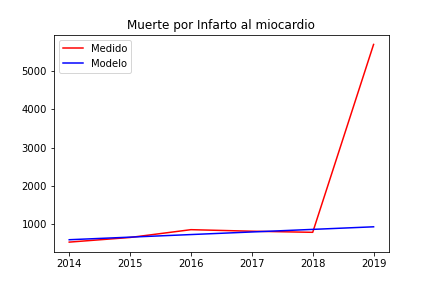
\includegraphics[scale=0.6]{Infarto.png}
    \caption{Modelo de las muertes en León por infartos comparado con los decesos registrados}
    \label{fig:my_label}
\end{figure}
\begin{itemize}
    \item \textbf{Muertes en León por diabetes}
\end{itemize}
A medida que fue recolectando los datos suficientes para generar una regresión lineal pude rescatar que en León se registraron 511, 501, 577, 606 y 59 muertes por diabetes entre el 2014 y 2018. Con la regresión lineal esperé que en 2019 se registraran 212 muertes cuando en realidad, filtrando la información del archivo del año 2019, se registraron 249, como se muestra en el siguiente gráfico:
\begin{figure}[H]
    \centering
    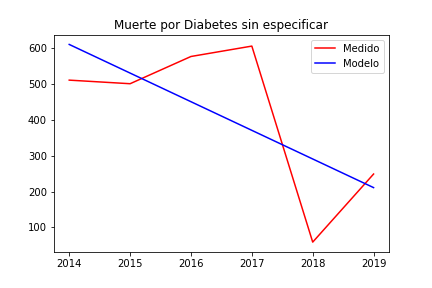
\includegraphics[scale=0.6]{Diabetes.png}
    \caption{Modelo de las muertes en León por diabetes comparado con los decesos registrados}
    \label{fig:my_label}
\end{figure}
\begin{itemize}
    \item \textbf{Muertes por síndrome de Dressler}
\end{itemize}
Este apartado es muy corto porque en realidad nadie murió en León durante el periodo 2014-2018, pero es un dato curioso que se puede obtener de los archivos. \\

\printbibliography
\end{document}